\nomenclature[]{VRP}{Vehicle Routing Problem}

\section{Scene Surveying}\label{sec:SceneSurveying}
This section outlines the algorithms that were explored to generate a set of routes for the UAVs that will be used to record sensor data at each of the grid points generated in the region of interest, which are generated using Algorithm \ref{alg:GridGeneration} described in the preceding section. We make some assumptions related to the solution of this problem:
\note{This list might not cover everything, come back to it}
\begin{itemize}
    \item Each UAV is assumed to have the same internal representation of the region of interest, namely the set of uniformly spaced grid points generated by Algorithm \ref{alg:GridGeneration}.
    \item Each UAV is assumed to have the ability to move between any pair of grid points unobstructed using the shortest possible path.
    \item UAVs are assumed to move with a fixed operational velocity, which can vary between UAVs.
    \item Each UAV may be equipped with different sensors to the others and it is assumed that sensing times may vary among the UAVs.
    \item Each UAV has a finite battery capacity which implies they have a finite amount of time that they can fly for before they need to recharge.
\end{itemize}

%Talk about how problem was transformed to TSP problem, took that and then divided up soln for mTSP.

The scene surveying problem that we would like to solve can be treated as an instance of the well-known \textit{Vehicle Routing Problem} (VRP), which was first described in a paper by \citeauthor{Dantzig1959TheProblem} \cite{Dantzig1959TheProblem}. This problem is a generalisation of the classic \textit{Travelling Salesman problem} (TSP). There are many variants and extensions to this problem, but it essentially asks for a set of routes to be assigned to the UAVs such that each point in the graph is visited exactly once, which minimises the total time taken to "service" each of the points. In our case, the service time is the time taken to record a sensor reading. We are interested solving this problem where the graph is defined by the grid of points that is generated using Algorithm \ref{alg:GridGeneration}. A formal definition of the VRP and its variants can be found in \cite{Toth2002TheProblem}.

\subsection{Simplified Problem}
\note{maybe change this to constrained problem or something similar}
We began by taking a simplified version of the full vehicle routing problem in order to explore possible solutions. This section expands on our published work in \cite{Smyth2018UsingDrones}, which summarises how this simplified problem was tackled. Rather than concern ourselves with the details of sensor sampling times and battery constraints, we first focused on designing a solution that can assign a set of routes to a homogeneous set of UAVs. 
%We assumed that service times add a fixed constant to the total time taken to perform the survey (and can hence be ignored) and we ignore the time added that the UAVs might need to recharge. 
The problem can be described as follows:
\\
\textit{Given a fully connected graph, $G$, to visit and $n$ RAV agents, find a subtour for each agent such that each point in $P \in G$ is visited exactly once by any agent in the system, with the objective of minimizing the longest time taken for any individual agent subtour, in order to minimize the time taken to carry out the survey.}
\\
This is simply the \textit{ multiple travelling salesman problem} (mTSP). 

%According to the number of distribution centers: single distribution center and multi-distribution center problem;
%According to the type of vehicle: single-vehicle type and multi-vehicle type problem;
%According to the characteristics of the task: pure send (take) cargo problems and loading and unloading mixing problem;
%According to whether the time constraints: no time window problem and time window problem;
%By vehicle loading: And the problem of non-full load;
%According to the optimization of the number of goals: a single objective and multi-objective problem;
%Vehicle and vehicle by the ownership of the points: the vehicle open problem and vehicle closure problems;
%By mastering the information of certainty: Sexual VRP and non-deterministic VRP problems;
%As can be seen from these classifications, solutions to the VRP problem are varied, each category 

\subsection{Proposed Solution for the Simplified Problem}
\note{Again maybe use constrained instead of simplified}
Due to the fact that the mTSP is at least as hard as the TSP, since it is a generalisation of the TSP, finding a polynomial time solution to the mTSP is not feasible. Given that there is no algorithm to solve the mTSP optimally in a polynomial time, we explored a number of sub-optimal solutions that take advantage of the highly structured nature of the uniformly spaced grid that we use in our instance of the problem. The usual trade-off between solution quality vs. time taken to find the solution motivated our choice of implemented algorithm, as we anticipated that the time taken to execute the planned routes may be comparable to the time taken to generate some solutions (the order of minutes or hours). For example, \cite{Hungerlander2018TheGrids} shows the results of using a Mixed Integer Linear Program (MILP) took hours to run for grid sizes that would be considered relatively small in our domain, which would exceed the amount of time taken to perform even a random solution. General details of solutions that can be applied to solve the mTSP and VRP can be found in Section <> of the literature review.

\subsubsection{Nearest Neighbor Algorithm}
There are four common heuristic algorithms that form the basis of most solutions to TSP and mTSP problems, which are stated in \cite{Johnson1997TheOptimization}: the \textit{nearest neighbor} algorithm, the \textit{greedy algorithm}, the \textit{Clarke-Wright} algorithm and the \textit{Christofides} algorithm. We began by implementing an algorithm which is a modification of a TSP solution based on the nearest-neighbor heuristic. Our reasoning is based on the following premises:
\begin{enumerate}
    \item The nearest-neighbor heuristic is a well-known heuristic that is straightforward to implement. It is known to provide good results to the TSP when the cost is defined as the Euclidean distance between points \cite{Johnson1995TheOptimization}, as in our use case.
    \item The nearest-neighbor solution to the TSP can be very easily modified to be applied to the mTSP.
    \item The nearest-neighbor heuristic is known to have a running time which is O($n^2$) \cite{Rosenkrantz1977AnProblem}, which means it can scale well to reasonably large problem instances compared to other algorithms which have a far worse performance complexity. For example, the Christofides algorithm is known to be within a factor of $\frac{3}{2}$ of the optimal solution, but its running time is O($n^3$) \cite{Christofides1976WORST-CASEPROBLEM}, which quickly becomes prohibitively long.
    %\item Partitioning a TSP solution can give very good mTSP solutions on the same graph.
\end{enumerate}

The nearest-neighbor heuristic algorithm for the multiple Travelling Salesman problem is shown in Algorithm \ref{alg:NNHeuristic}.

\begin{algorithm}
\caption{The Nearest-Neighbor Solution to the mTSP Problem}
\label{alg:NNHeuristic}
\begin{algorithmic}[1]
\renewcommand{\algorithmicrequire}{\textbf{Input:}}
\renewcommand{\algorithmicensure}{\textbf{Output:}}

\REQUIRE$ \newline k \quad \text{ The number of UAVs in the mTSP }
\newline way\_points \quad \text{ The set of points the UAVs must visit }
\newline cost(i,j) \quad \text{ The function giving the cost of travelling from node i to node j }
$
\ENSURE $ \newline UAV\_routes \quad \text{A key-value data structure mapping UAVs to their corresponding routes.}
$

\hfill\pagebreak

%\noindent\textbf{\textit{\noindent Initialization} :}\\
\STATE UAV\_routes$\leftarrow$empty key-value container
\STATE visited\_points$\leftarrow$empty array
\STATE remaining\_points\_to\_visit$\leftarrow$way\_points
\FOR{each agent in agents:}
%\quad 
\STATE Initialise path of agent as empty array in UAV\_routes
\ENDFOR

current\_agent\_index$\leftarrow$0\\
%current\_agent$\leftarrow$agents.get(current\_agent\_index)\\
\hfill\pagebreak
\WHILE {pointsToVisit is not empty}
\STATE agent\_position $\leftarrow$ last value in agent\_paths.get(current\_agent\_index)
\STATE nearest\_neighbor$\leftarrow$\(\displaystyle \min_{neighbor \in points\_to\_visit}\)cost(agent\_position, neighbor)
\STATE Update current\_agent value in agent\_paths to include nearest\_neighbor
\STATE Add nearest\_neighbor to visited\_points.
\STATE Remove nearest\_neighbor from remaining\_points\_to\_visit.
\STATE current\_agent\_index$\leftarrow$(currentAgentIndex+1) $\mathbf{mod}$$\vert$List of Agents$\vert$

%\STATE currentAgent$\leftarrow$agents.get(currentAgentIndex)


\ENDWHILE
\RETURN UAV\_routes
\end{algorithmic} 
\end{algorithm}


\begin{wrapfigure}{r}{0.45\textwidth}
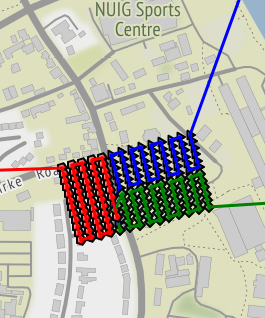
\includegraphics[width=0.45\textwidth]{Chapters/MultiAgentCoverage/Figs/RAVRoutingNUIGCropped.png}
\caption{NN heuristic encourages the creation of optimal sub-tours, which are assigned to each UAV}
\label{fig:NNPartitioning}
\end{wrapfigure}
The algorithm can be seen to be a very straightforward extension of the single agent NN algorithm. The while loop iteratively cycles through the list of UAVs and assigns the nearest non-assigned neighbor to the next UAVs partially assembled route. Since we run this algorithm over a uniformly-spaced grid, it builds agent routes in a lawn-cutting pattern, which intuitively will provide good results as long as the routes do not begin to overlap. The idea is to take the NN algorithm TSP solution and apply it exhaustively in a round-robin manner, so that each UAV is encouraged to find a non-overlapping optimal sub-tour. These non-overlapping optimal sub-tours partition the region and therefore offer a solution to the mTSP. Section 4 of \cite{Hungerlander2018TheGrids} gives an insight to how optimal solutions can be found for a uniformly spaced rectangular grid when UAVs are assumed to start in the corners of the rectangle, which provides further motivation to using algorithm \ref{alg:NNHeuristic}. In practice non-overlapping optimal sub-tours are not found, but solutions may come close, as illustrated in figure \ref{fig:NNPartitioning}. Since sometimes the solutions found by the algorithm are not always well-balanced, we propose to iteratively re-run the algorithm after a set interval in order to update the solution to ensure that no UAV is idle while others are doing work. This also ensures redundancy in the system - if a UAV stops operating, it's uncompleted work will be re-assigned to the others.

\note{Not sure if worth mentioning lower bound of cost for this algo is 1/noUAVs}
\note{might be worth mentioning that it would be ideal to add the next grid point to whichever agent has the shortest route so far}



\subsubsection{Analysis of the NN algorithm}
\note{The justification behind this choice of algo is a bit weak, might be worth running tests on file:///C:/Users/13383861/Downloads/graphsOR18.pdf}


The results and analysis of applying the NN heuristic algorithm to the symmetric Euclidean TSP and mTSP are well documented and we will not go into great detail repeating the results here. Instead, we refer the reader to the chapter ``The travelling salesman problem: A case study'' of \cite{Aarts:1997:LSC:549160}, written by \citeauthor{Johnson1995TheOptimization}, which provides a comparison of the NN heuristic to other heuristic algorithms. They compare solutions with the standard Held-Karp lower bound \cite{Held1962AProblems} using a standardised library of Travelling Salesman Problems, TSPLIB \cite{TSPLIB}. Rather than provide tables of results showing the performance of the NN heuristic algorithm on standard benchmark data sets such as TSPLIB, we instead focus on the results for the domain we are most interested in, which is a connected graph defined by a uniformly spaced set of grid points. We found that the algorithm performed best when the UAVs used regions that have multiple axes of symmetry. Rectangular regions in particular yield scalable, high-quality solutions, as shown in the figures in table \ref{table:NNAlgoResultsRect}. This corresponds to the optimal performance configuration suggested in \cite{Hungerlander2018TheGrids}. We evaluated solutions both qualitatively and  quantitatively. We found that UAV starting points are a critical factor in solution quality, which again is in line with the findings in \cite{Hungerlander2018TheGrids}. Tables \ref{table:NNAlgoResultsRect}, \ref{table:NNAlgoResultsTri}, \ref{table:NNAlgoResultsHex} and \ref{table:NNAlgoResultsIrregular} illustrate some of the results, with the configuration of each listed below.\\

\textbf{Rectangular Region}
\\Spacing between grid points: 23m in latitude, 25m in longitude.
\\Bounding rectangle coordinates: (53.2781933786, -9.0671226391), (53.2803800539, -9.067182416), (53.2804392784, -9.0611222377), (53.2782526061, -9.0610624609)
\\
\begin{table}[h!]
  \centering
  \begin{tabular}{ | c | m{5cm} | }
    \hline
    Planned UAV Routes & Route Lengths (metres) \\
    \hline
    
    %single UAV
    \begin{minipage}[c][53mm][c]{.6\textwidth}
      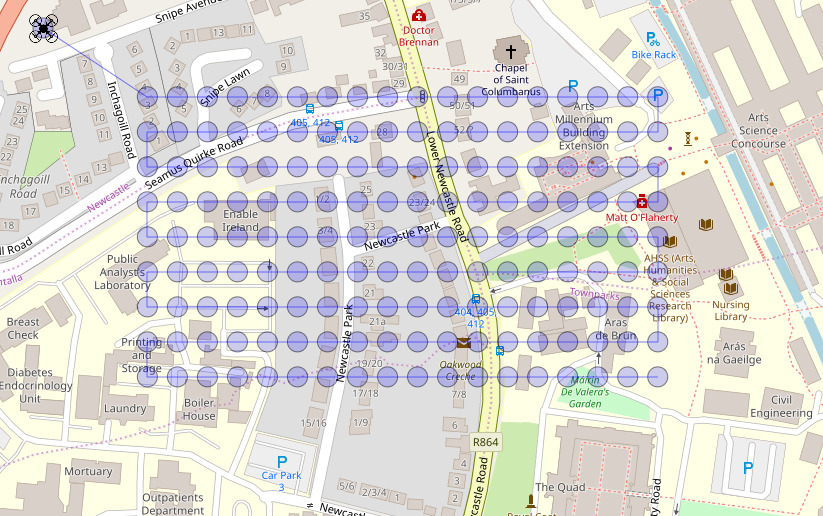
\includegraphics[width=\linewidth, height=51mm]{Chapters/MultiAgentCoverage/MultipleTravellingSalesman/Figs/Rectangle/SingleAgent.PNG}

    \end{minipage}
    &
    \begin{itemize}[leftmargin=*]
      \item[] UAV 1 (blue): 3576.6
    \end{itemize}
    \\
    \hline
    %two UAV
    \begin{minipage}[c][53mm][c]{.6\textwidth}
      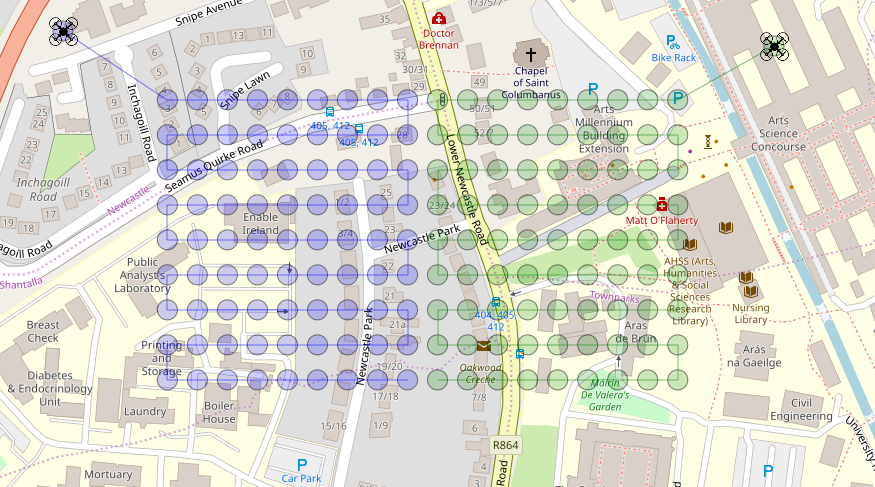
\includegraphics[width=\linewidth, height=51mm]{Chapters/MultiAgentCoverage/MultipleTravellingSalesman/Figs/Rectangle/TwoAgent.PNG}
    \end{minipage}
    &
    \begin{itemize}[leftmargin=*]
        \item[] UAV 1 (blue): 1825.8
        \item[] UAV 2 (green): 1836.3
    \end{itemize}
    \\
    \hline
    
    %three UAV
    \begin{minipage}[c][53mm][c]{.6\textwidth}
      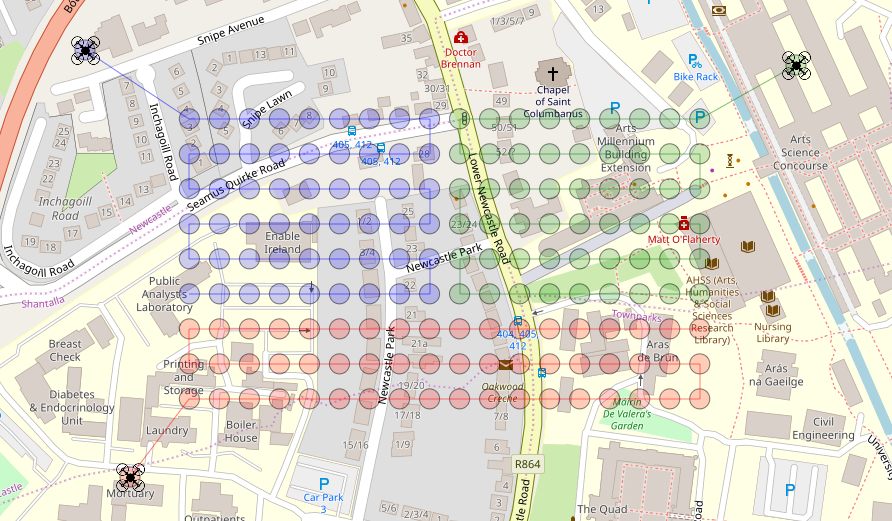
\includegraphics[width=\linewidth, height=51mm]{Chapters/MultiAgentCoverage/MultipleTravellingSalesman/Figs/Rectangle/ThreeAgent.PNG}
    \end{minipage}
    &
    \begin{itemize}[leftmargin=*]
    \item[] UAV 1 (blue): 1235.1
    \item[] UAV 2 (green): 1245.6
    \item[] UAV 3 (red): 1215.9
    \end{itemize}
    \\
    \hline
    
    %Four UAV
    \begin{minipage}[c][53mm][c]{.6\textwidth}
      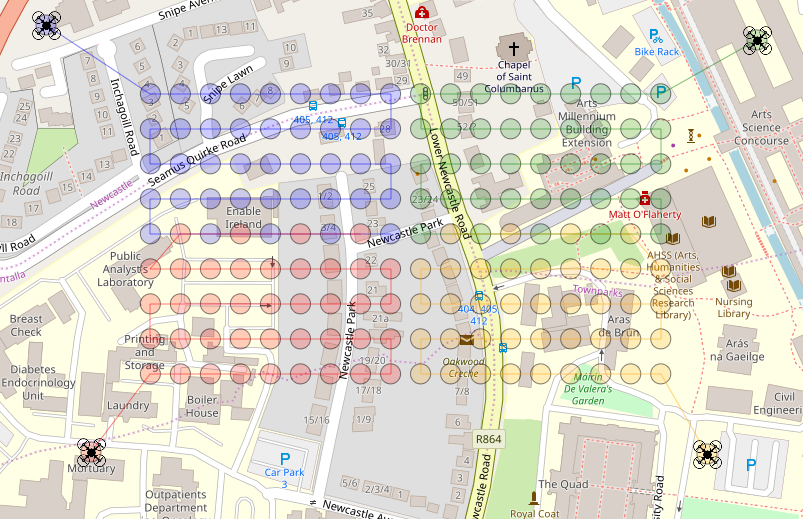
\includegraphics[width=\linewidth, height=51mm]{Chapters/MultiAgentCoverage/MultipleTravellingSalesman/Figs/Rectangle/FourAgent.PNG}
    \end{minipage}
    &
    \begin{itemize}[leftmargin=*]
    \item[] UAV 1 (blue): 1038.3
    \item[] UAV 2 (green): 1048.8
    \item[] UAV 3 (red): 994.5
    \item[] UAV 4 (yellow): 990.5
    \end{itemize}

    \\
    \hline
  \end{tabular}
  \caption{Results of applying NN algorithm to a rectangular region}\label{table:NNAlgoResultsRect}
\end{table}


\textbf{Triangular Region}
\\Spacing between grid points: 23m in latitude, 25m in longitude.
\\Bounding rectangle coordinates: (53.2781933786, -9.0671226391), (53.2782526061, -9.0610624609), (53.2803800539, -9.06409255)
\\
\begin{table}[h!]
  \centering
  \begin{tabular}{ | c | m{5cm} | }
    \hline
    Planned UAV Routes & Route Lengths (metres) \\
    \hline
    
    %single UAV
    \begin{minipage}[c][57mm][c]{.6\textwidth}
      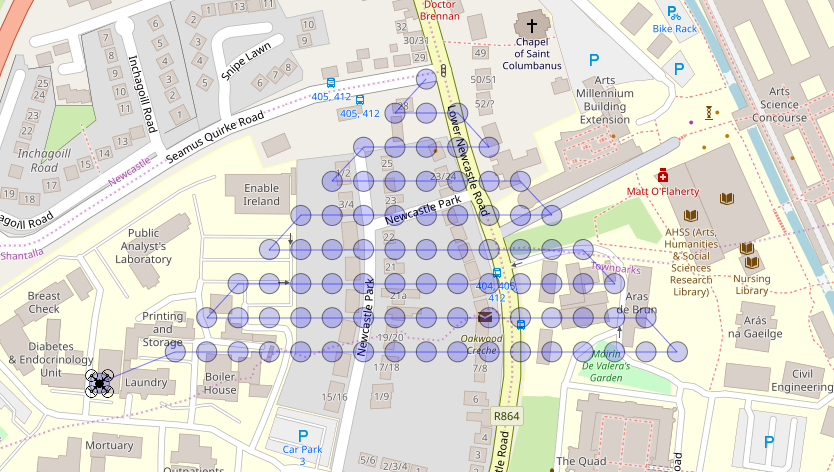
\includegraphics[width=\linewidth, height=55mm]{Chapters/MultiAgentCoverage/MultipleTravellingSalesman/Figs/Triangle/OneRAV.PNG}
    \end{minipage}
    &
    \begin{itemize}[leftmargin=*]
      \item[] UAV 1 (blue): 1940.6
    \end{itemize}
    \\
    \hline
    %two UAV
    \begin{minipage}[c][57mm][c]{.6\textwidth}
      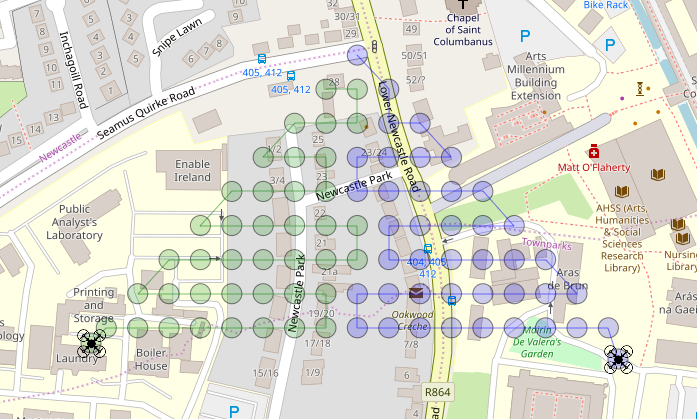
\includegraphics[width=\linewidth, height=55mm]{Chapters/MultiAgentCoverage/MultipleTravellingSalesman/Figs/Triangle/TwoRAV.PNG}
    \end{minipage}
    &
    \begin{itemize}[leftmargin=*]
        \item[] UAV 1 (blue): 930.7
        \item[] UAV 2 (green): 971.8
    \end{itemize}
    \\
    \hline
    
    %three UAV
    \begin{minipage}[c][57mm][c]{.6\textwidth}
      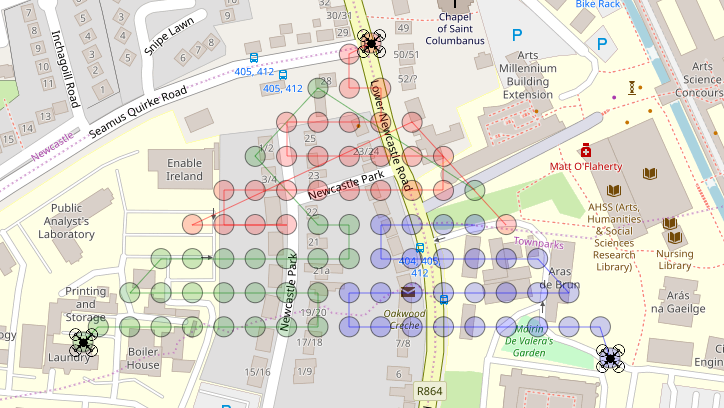
\includegraphics[width=\linewidth, height=55mm]{Chapters/MultiAgentCoverage/MultipleTravellingSalesman/Figs/Triangle/ThreeRAV.PNG}
    \end{minipage}
    &
    \begin{itemize}[leftmargin=*]
    \item[] UAV 1 (blue): 812.7
    \item[] UAV 2 (green): 621.6
    \item[] UAV 3 (red): 883.4
    \end{itemize}
    \\
    \hline
  \end{tabular}
  \caption{Results of applying NN algorithm to a triangular region}\label{table:NNAlgoResultsTri}
\end{table}


\textbf{Hexagonal Region}
\\Spacing between grid points: 32m in latitude, 38m in longitude.
\\Bounding rectangle coordinates: (53.2782526061, -9.0610624609), (53.2803800539, -9.06409255), (53.2781933786, -9.0671226391), (53.27621, -9.0671226391), (53.27402, -9.06409255), (53.27615, -9.0610624609)
\\


\begin{table}[h!]
  \centering
  \begin{tabular}{ | c | m{5cm} | }
    \hline
    Planned UAV Routes & Route Lengths (metres) \\
    \hline
    
    %single UAV
    \begin{minipage}[c][68mm][c]{.6\textwidth}
      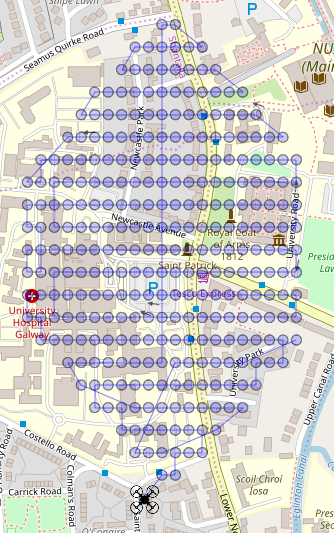
\includegraphics[width=\linewidth, height=66mm]{Chapters/MultiAgentCoverage/MultipleTravellingSalesman/Figs/Hexagon/OneRAV.PNG}
    \end{minipage}
    &
    \begin{itemize}[leftmargin=*]
      \item[] UAV 1 (blue): 7247.2
    \end{itemize}
    \\
    \hline
    %two UAV
    \begin{minipage}[c][68mm][c]{.6\textwidth}
      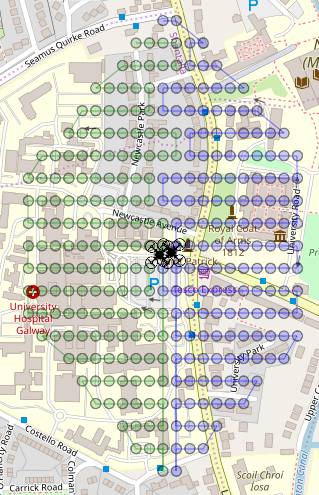
\includegraphics[width=\linewidth, height=66mm]{Chapters/MultiAgentCoverage/MultipleTravellingSalesman/Figs/Hexagon/TwoRAV.PNG}
    \end{minipage}
    &
    \begin{itemize}[leftmargin=*]
        \item[] UAV 1 (blue): 3544.2
        \item[] UAV 2 (green): 3587.4
    \end{itemize}
    \\
    \hline
    
    %three UAV
    \begin{minipage}[c][68mm][c]{.6\textwidth}
      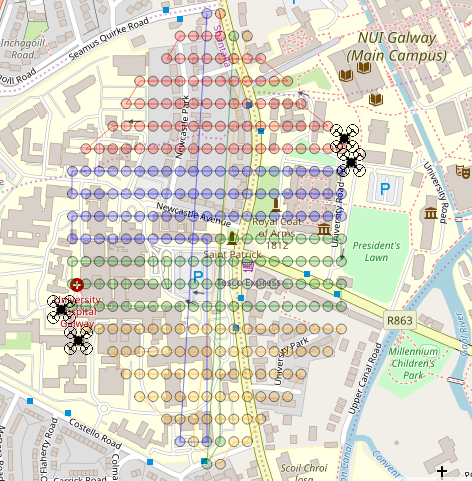
\includegraphics[width=\linewidth, height=66mm]{Chapters/MultiAgentCoverage/MultipleTravellingSalesman/Figs/Hexagon/FourRAV.PNG}
    \end{minipage}
    &
    \begin{itemize}[leftmargin=*]
    \item[] UAV 1 (blue): 1629.6
    \item[] UAV 2 (green): 2435.6
    \item[] UAV 3 (red): 2412.0
    \item[] UAV 4 (yellow): 2245.9
    \end{itemize}
    \\
    \hline
  \end{tabular}
  \caption{Results of applying NN algorithm to a hexagonal region}\label{table:NNAlgoResultsHex}
\end{table}


\textbf{Irregular Region}
\\Spacing between grid points: 20m in latitude, 20m in longitude.
\\Bounding rectangle coordinates: (53.28048,-9.069021), (53.28189,-9.066017), (53.28009,-9.065223), (53.28192,-9.064128), (53.28026,-9.061725), (53.27923,-9.063957), (53.27846,-9.063721), (53.27712,-9.063721), (53.27626,-9.060159), (53.27516,-9.061124), (53.27412,-9.061425), (53.27362,-9.061425), (53.2735,-9.062562), (53.27456,-9.06327), (53.27416,-9.064794), (53.27495,-9.06754), (53.27456,-9.067841), (53.27354,-9.067605), (53.27346,-9.06857), (53.27466,-9.06872), (53.2752,-9.06827), (53.27583,-9.070008), (53.27571,-9.07093), (53.27545,-9.074385), (53.27581,-9.074149), (53.27609,-9.07445), (53.2788,-9.069986), (53.27951,-9.069793), (53.28116,-9.071081), (53.28148,-9.069686)
\\
\begin{table}[h!]
  \centering
  \begin{tabular}{ | c | m{5cm} | }
    \hline
    Planned UAV Routes & Route Lengths (metres) \\
    \hline
    
    %single UAV
    \begin{minipage}[c][68mm][c]{.6\textwidth}
      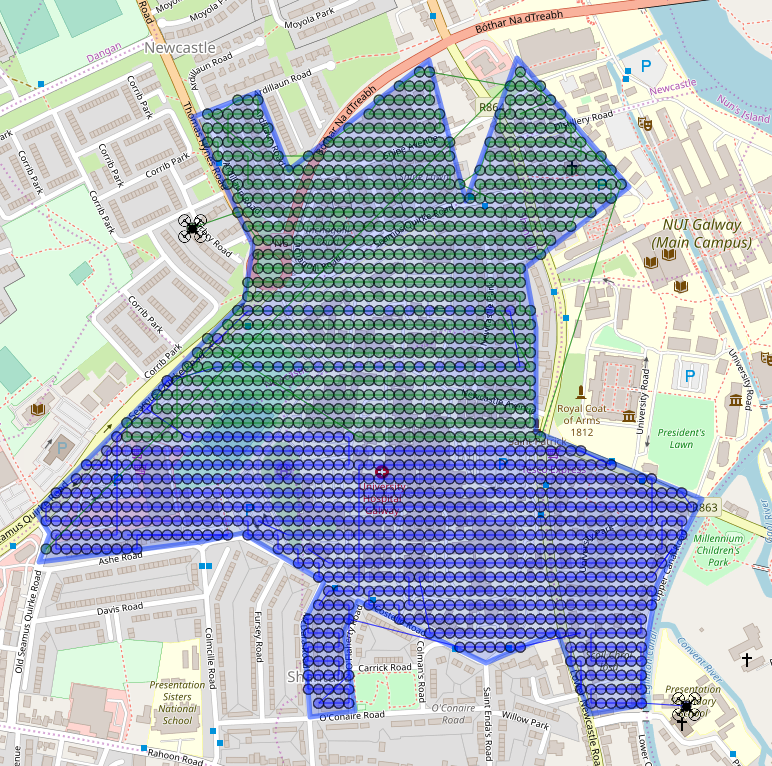
\includegraphics[width=\linewidth, height=66mm]{Chapters/MultiAgentCoverage/MultipleTravellingSalesman/Figs/IrregularRegion/TwoRAV.PNG}
    \end{minipage}
    &
    \begin{itemize}[leftmargin=*]
       \item[] UAV 1 (blue): 14268.6
        \item[] UAV 2 (green): 13393.6
    \end{itemize}
    \\
    \hline
    %two UAV
    \begin{minipage}[c][68mm][c]{.6\textwidth}
      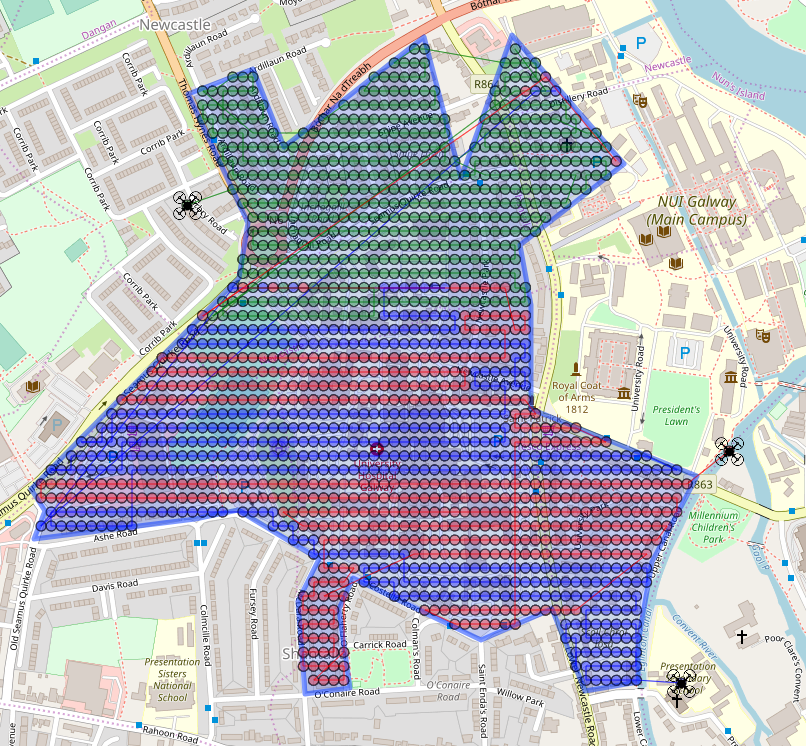
\includegraphics[width=\linewidth, height=66mm]{Chapters/MultiAgentCoverage/MultipleTravellingSalesman/Figs/IrregularRegion/ThreeRAV.PNG}
    \end{minipage}
    &
    \begin{itemize}[leftmargin=*]
        \item[] UAV 1 (blue): 8879.8
        \item[] UAV 2 (green): 9596.4
        \item[] UAV 3 (green): 9433.4
    \end{itemize}
    \\
    \hline
    
    %three UAV
    \begin{minipage}[c][68mm][c]{.6\textwidth}
      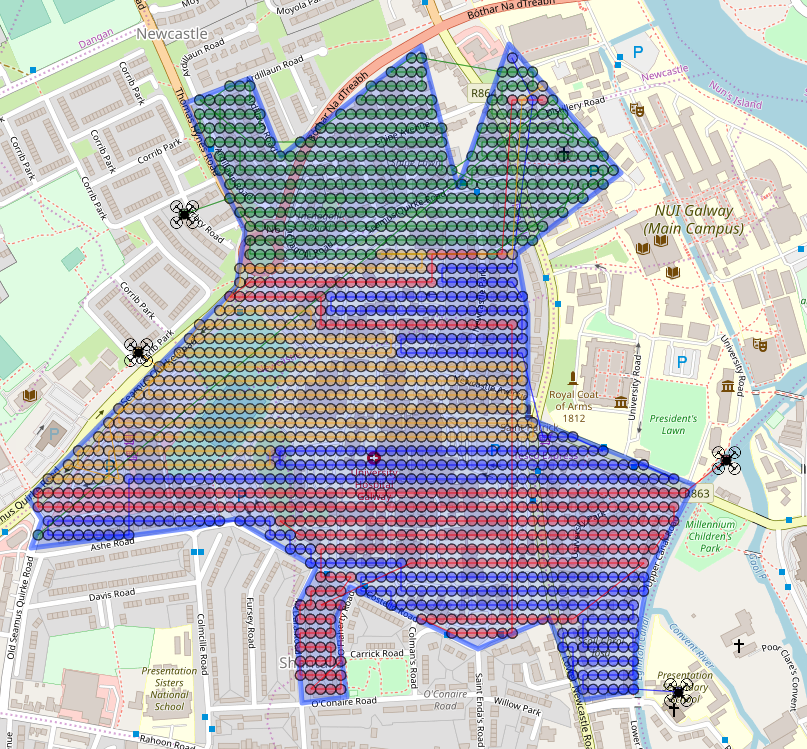
\includegraphics[width=\linewidth, height=66mm]{Chapters/MultiAgentCoverage/MultipleTravellingSalesman/Figs/IrregularRegion/FourRAVSecondAttempt.PNG}
    \end{minipage}
    &
    \begin{itemize}[leftmargin=*]
    \item[] UAV 1 (blue): 7673.2
    \item[] UAV 2 (green): 6354.0
    \item[] UAV 3 (red): 6860.6
    \item[] UAV 4 (yellow): 6368.8
    \end{itemize}
    \\
    \hline
  \end{tabular}
  \caption{Results of applying NN algorithm to an irregular region}\label{table:NNAlgoResultsIrregular}
\end{table}
\pagebreak



































%\subsubsection{Proof of Lower Bound of Nearest Neighbor Solution}
%Let O be a tour that is an optimal solution to the Travelling Salesperson Problem (TSP) for  a graph G(V, E), where E $\subseteq$ V $\times$ V, with a cost function c$(p_i, p_j)$ defined for all $(p_i, p_j)$ $\in$ E and an induced cost function 
%C($T$) = $\sum\limits_{(p_i, p_j)\in }$C$(p_i, p_j)$ defined for any tour $T$ of G.
%The optimal tour O is an ordered tuple (($p_i, p_j$), ($p_j, p_k$),..., ($p_m, p_n$)) $\subseteq$ E which satisfies:
%\[
%Cost(O) =  \min_{e \subseteq E}\sum_{(p_i, p_j) \in e} c(p_i, p_j) 
%\]
%with the constraint that each $p_i \in$ V must be visited exactly once. This means that O is a Hamiltonian tour of G of minimal cost. 
%\\
%For any partition ($T_1, T_2, ..., T_m$) of an arbitrary tour T', we find:

%\[\text{Cost}(T')=\sum\limits_{k=1}^{m}\sum\limits_{(p_i, p_j)\in T_k} \text{cost}(p_i, p_j) \leq m \times \max_{T_k \in T}
%\sum\limits_{(p_i, p_j)\in T_k}c(p_i, p_j) = 
%m \times \max_{T_k \in T} \text{Cost}(T_k)
%\]

%\noindent Since Cost(O) $\leq$ Cost(T'), for the partition determined by any solution to the TSP, we find that for any solution S to mTSP consisting of the partition ($S_1, S_2, ...,S_m$) for each of the m agents:\\

%\[
%Cost(T)
%\leq Cost(S) \leq  m \times
%\max_{S_k \in S}
%\sum\limits_{(p_i, p_j)\in S_k}C(p_i, p_j)) = Cost of MTS solution, S.
%\]
%This means we can use a solution of the standard Traveling Salesperson problem as a lower bound for comparison with Algorithm \ref{alg:agentRoutesEdited}. For example, the Held-Karp algorithm gives a well-known lower bound when dealing with a metric space \cite{VALENZUELA1997157}.

%We explored a number of solutions to this 



\subsubsection{}